% ICAISC 2027 submission -- Springer LNAI (llncs class)
% Double-blind: keep the anonymous author block until camera-ready.
% Overleaf: New Project -> Upload Project (this zip). llncs.cls and splncs04.bst
% are built into Overleaf's TeX Live, so no extra files are needed there.
\documentclass[runningheads]{llncs}

\usepackage[T1]{fontenc}
\usepackage{graphicx}
\usepackage{amsmath,amssymb}
\usepackage{booktabs}
\usepackage{multirow}
\usepackage{xcolor}
\usepackage{url}
\usepackage[hidelinks]{hyperref}
\renewcommand\UrlFont{\color{blue}\rmfamily}

% ---- writing helpers (delete before submission) --------------------------
\newcommand{\TODO}[1]{\textcolor{red}{[TODO: #1]}}
\newcommand{\RES}[1]{\textcolor{blue}{[#1]}}   % numbers filled in from results/
% ---------------------------------------------------------------------------

% notation
\newcommand{\Elow}{\underline{E}}
\newcommand{\Ehigh}{\overline{E}}
\newcommand{\mulow}{\underline{\mu}}
\newcommand{\muup}{\overline{\mu}}

\begin{document}

\title{Whose Gesture Is It? Uncertainty-Aware Interval Type-2 Fuzzy
Engagement Gating for Gesture Commands to a Quadruped Robot in Crowds}
\titlerunning{Interval Type-2 Engagement Gating for Gesture Commands in Crowds}

% ---- ANONYMOUS for review. Real block is commented out below. -------------
\author{Anonymous Author(s)}
\authorrunning{Anonymous}
\institute{Anonymous Institution}
% \author{Kaveeshwara Bandara \and Rivikula Fernando \and Agra Navarathna
%   \and Himasara Kulasinghe \and Lasan Perera}
% \authorrunning{K. Bandara et al.}
% \institute{Faculty of Engineering, University of Moratuwa, Sri Lanka}

\maketitle

\begin{abstract}
Gesture interfaces let people command mobile robots where speech fails, but
in shared spaces they answer \emph{what} a hand is doing and not \emph{whose}
hand it is or whether the gesture is meant for the robot. A bystander waving
at a friend can therefore stop or start the robot. We present a per-person
engagement gate for gesture commands on a quadruped robot that uses an RGB-D
camera mounted on the robot. Every visible person is tracked; hands are attributed to
bodies and classified per person; and a two-layer fuzzy system decides whether
each gesture is executed. The first layer estimates engagement from distance,
approach speed, body and head orientation and eye gaze; the second combines
engagement with gesture confidence. In the Interval Type-2 (IT2) variant, the
footprint of uncertainty of every input is set at run time from that person's
measured perception uncertainty, and the decision uses the lower bound of the
type-reduced engagement interval, so a person who is hard to see must look
more clearly engaged before being obeyed. We evaluate on
\RES{N} recordings with a Unitree Go2 and \RES{P} participants
(\RES{E} hand-labelled gesture episodes), comparing gesture-only,
nearest-person, gaze-only, learned, Type-1 and IT2 policies on identical
inputs. \RES{One sentence with the headline result: e.g. while the robot
walked, IT2 reduced bystander false triggers from X\% to Y\% at Z\% commander
recall.}
\keywords{Interval type-2 fuzzy logic \and Human--robot interaction \and
Gesture recognition \and Engagement estimation \and Quadruped robot}
\end{abstract}

\section{Introduction}
\label{sec:intro}

Hand gestures are a natural way to command a mobile robot in places where
speech is unreliable, such as a busy lobby, a laboratory or a caf\'e.
Legged robots are increasingly deployed in exactly these spaces, and
off-the-shelf pipelines now detect and classify hand gestures in real time on
modest hardware~\cite{zhang2020mediapipehands,kapitanov2024hagrid}. Most
gesture interfaces, however, assume a single user standing in front of the
robot: a hand is detected, classified and mapped to a velocity command. In a
crowd this assumption breaks. Several people are in view, many of them
gesture to each other, and the robot cannot tell a command from a
conversation. A bystander's open palm stops the robot; a fist meant for a
friend sends it walking.

The question a gesture interface must answer in a shared space is therefore
not only \emph{which} gesture is shown, but \emph{who} is showing it and
\emph{whether it is addressed to the robot}. We formulate three requirements:
\begin{enumerate}
\item[R1] gestures from different people are recognised and attributed to
  the right person, even when they occur at the same time;
\item[R2] only gestures addressed to the robot are executed;
\item[R3] the same person is ignored when they turn and gesture to someone
  else.
\end{enumerate}

Humans resolve this with nonverbal cues: people who address someone face
them, look at them and stand within a social distance~\cite{hall1966hidden,
kendon1990conducting}. These cues are easy to state as linguistic rules
(``\emph{if} a person is facing the robot \emph{and} is at a social distance
\emph{then} they are engaged''), which makes fuzzy logic a natural model.
The difficulty is that the cues are measured from a moving robot: depth
readings have holes and edge errors on people, gaze is only resolvable at
short range, and orientation estimates degrade with occlusion and motion
blur. A
Type-1 fuzzy system treats every reading as exact. An Interval Type-2 (IT2)
system can represent how much each reading should be trusted, but in most
applications its footprint of uncertainty (FOU) is fixed at design time.

We propose an engagement gate in which the FOU of every input is driven at
run time by the measured uncertainty of that input for that person. When a
person is clearly visible the IT2 system behaves like its Type-1 counterpart;
when they are far away, partly occluded or turning, the engagement interval
widens and the decision, taken on its lower bound, becomes conservative. The
contributions of this paper are:
\begin{itemize}
\item a per-person perception pipeline for a quadruped robot that attributes
  gestures to individuals and estimates distance, approach speed,
  orientation and gaze, each with an explicit uncertainty, from a single
  RGB-D camera mounted on the robot;
\item a two-layer fuzzy engagement gate for gesture commands, and an IT2
  variant whose FOU is set per person and per frame from measured perception
  uncertainty, reducing exactly to the Type-1 system when uncertainty is
  zero;
\item an evaluation on a real Unitree Go2 in stationary and walking
  scenarios with several people, comparing gesture-only, nearest-person,
  gaze-only, learned, Type-1 and IT2 policies on identical inputs, with an
  analysis of where measured uncertainty helps.
\end{itemize}

The remainder of the paper is organised as follows. Section~\ref{sec:background}
reviews IT2 fuzzy systems, Section~\ref{sec:related} discusses related work,
Section~\ref{sec:method} describes the method, Section~\ref{sec:experiments}
the experimental setup, Section~\ref{sec:results} the results, and
Section~\ref{sec:discussion} limitations and future work.

\section{Background: Interval Type-2 Fuzzy Systems}
\label{sec:background}

A Type-1 fuzzy set assigns each input $x$ a crisp membership
$\mu(x)\in[0,1]$~\cite{zadeh1975linguistic}. When the shape or position of
that set is itself uncertain, a Type-2 set assigns a fuzzy membership
instead. In the interval case, every primary membership is an interval
$[\mulow(x),\muup(x)]$, and the region between the lower and upper membership
functions is the footprint of uncertainty
(FOU)~\cite{liang2000it2,mendel2006it2simple}.

A common way to build an IT2 set is a Gaussian with an uncertain mean
$m\in[m_1,m_2]$ and fixed spread $s$:
\begin{equation}
\muup(x)=
\begin{cases}
\mathcal{N}(x;m_1,s) & x<m_1\\
1 & m_1\le x\le m_2\\
\mathcal{N}(x;m_2,s) & x>m_2
\end{cases}
\qquad
\mulow(x)=\min\{\mathcal{N}(x;m_1,s),\,\mathcal{N}(x;m_2,s)\},
\label{eq:um-gauss}
\end{equation}
where $\mathcal{N}(x;m,s)=\exp\!\big(-\tfrac12((x-m)/s)^2\big)$. The width
$m_2-m_1$ controls how much the system hedges; when it is zero the set
collapses to a Type-1 Gaussian.

For a rule base with consequents $y_i$, each rule $i$ fires with an interval
$[\underline{f}_i,\overline{f}_i]$ obtained by applying a t-norm to the lower
and to the upper memberships of its antecedents. Type reduction computes the
centroid interval
\begin{equation}
y_l=\min_{f_i\in[\underline{f}_i,\overline{f}_i]}
  \frac{\sum_i f_i y_i}{\sum_i f_i},\qquad
y_r=\max_{f_i\in[\underline{f}_i,\overline{f}_i]}
  \frac{\sum_i f_i y_i}{\sum_i f_i},
\label{eq:km}
\end{equation}
which the Karnik--Mendel (KM) procedure finds exactly by locating one switch
point in the sorted consequents~\cite{karnik2001centroid}. A crisp output is
usually $(y_l+y_r)/2$, but the interval itself is informative: its width
reflects how much the input uncertainty affects the conclusion~\cite{wu2002bounds}.
IT2 controllers have been used in mobile robotics to cope with noisy
sensors and changing environments~\cite{hagras2004hierarchical}, typically
with an FOU chosen offline. In this work the FOU width is an online signal.

\section{Related Work}
\label{sec:related}

\paragraph{Engagement and addressee estimation.}
Engagement, the process by which participants start, maintain and end their
connection with each other, has long been studied in human--robot
interaction~\cite{sidner2005engagement}. Robots infer it from gaze, head
orientation, body posture and proximity~\cite{rich2010recognizing,
foster2017engagement}, and multi-party systems must additionally decide whom
they are interacting with~\cite{bohus2009multiparty,vazquez2017towards}.
Gaze in particular is a strong signal of attention and
address~\cite{admoni2017gaze}. Fuzzy models have been used for this problem:
Mu\~noz-Salinas et al.~\cite{munoz2005fuzzy} estimated each tracked person's
interest in interacting with a robot from distance, angle and face
orientation with a Type-1 fuzzy system, and Yun et al.~\cite{yun2012intention}
used a fuzzy engagement model to select which of several people a robot
should attend to. Our Layer~1 follows the same intuition. These systems,
however, decide where the robot directs its attention rather than whether a
command should be executed, and they treat perception as exact.

\paragraph{Gesture control of legged robots.}
Hand- and body-gesture interfaces have been built for quadrupeds, ranging from
deep-learning hand-gesture recognition for commanding a quadruped in 3D
space~\cite{hyperpalm2022} to combined body and hand gesture interfaces
evaluated with users~\cite{quadgesture2024}. They report good recognition
accuracy but assume one operator in front of the robot. A recent systematic
review of proactive robots in human groups finds that most systems make this
single-individual assumption~\cite{grouprobots2026review}.

\paragraph{Gaze estimation from a robot camera.}
Appearance-based gaze estimation has progressed with large in-the-wild
datasets~\cite{zhang2019mpiigaze,kellnhofer2019gaze360}, but accuracy drops
quickly as the eye region shrinks. On a robot camera, eyes span only a few
pixels beyond two to three metres, so gaze is informative at short range and
head and body orientation must take over further away. This
distance-dependent reliability is exactly what an uncertainty-aware fusion
should capture.

\paragraph{Type-2 fuzzy logic under sensor noise.}
IT2 fuzzy systems are motivated by uncertainty in measurements and in the
meaning of linguistic terms~\cite{mendel2006it2simple}, and have been applied
to robot control~\cite{hagras2004hierarchical}. The FOU is usually tuned
offline or calibrated from a fixed sensor noise model. We instead let the FOU
of each input follow that input's measured uncertainty for each person and
each frame.

\paragraph{Positioning.}
To our knowledge no prior work combines (i)~per-person gesture attribution
and command gating in a crowd, (ii)~an IT2 engagement model whose FOU is
driven at run time by measured perception uncertainty, including
distance-dependent gaze reliability, and (iii)~an evaluation on a real
quadruped against gesture-only, nearest-person, gaze-only, learned and
Type-1 policies. We do not claim fuzzy engagement estimation itself as new.

\section{Method}
\label{sec:method}

\TODO{Pipeline figure (Fig.~\ref{fig:pipeline}): camera $\rightarrow$
per-person perception $\rightarrow$ Layer 1 $\rightarrow$ Layer 2
$\rightarrow$ arbitration $\rightarrow$ Move/StopMove.}

\subsection{Per-person perception}
Colour and depth frames from an Orbbec RGB-D camera mounted on the robot
\TODO{model, resolution, fps}, with depth aligned to colour, are processed on
a laptop. A
multi-person pose model~\cite{bazarevsky2020blazepose} returns body landmarks
for up to six people, which are tracked across frames by nearest shoulder
centre. For each person $p$ at time $t$ we compute:
\begin{itemize}
\item \emph{distance} $d$, the median depth sampled on the shoulder and hip
  landmarks; its uncertainty $\sigma_d$ combines the spread of those samples,
  the fraction of invalid depth pixels and the temporal standard deviation.
  When depth is missing, $d$ falls back to apparent shoulder width with a
  larger $\sigma_d$;
\item \emph{approach speed} $v$, the smoothed negative derivative of $d$;
\item \emph{facing} $f\in[0,1]$, combining head yaw (nose position between
  the ears, weighted by eye visibility) and body yaw (shoulder depth
  difference); $\sigma_f$ grows as landmark visibility drops and as $f$
  fluctuates;
\item \emph{gaze} $g\in[0,1]$, from iris landmarks relative to the eye
  corners combined with head yaw; $\sigma_g$ grows as the inter-ocular
  distance in pixels shrinks, so gaze becomes uninformative at long range.
  \TODO{exact formula once implemented}
\end{itemize}
Hands are detected with~\cite{zhang2020mediapipehands} and assigned to the
person whose wrist landmark is nearest, normalised by shoulder width (at most
0.7 shoulder widths). Each hand is classified by an 18-class keypoint
classifier~\TODO{cite source / training data}; labels are smoothed per person
by majority vote over seven frames, and confidence $c$ is the mean softmax
probability of the winning label times its vote share.

\subsection{Layer 1: engagement}
Distance uses three sets following Hall's proxemic
zones~\cite{hall1966hidden} (NEAR, MID, FAR); facing and gaze have LOW and
HIGH; approach speed has AWAY, STILL and TOWARD. The rule base
\TODO{final rule table, e.g.\ Table~\ref{tab:rules}} maps these to
singleton engagement consequents, e.g.\ \emph{if facing is HIGH and distance
is MID then $E=0.85$}; \emph{if approach is AWAY then $E=0.10$}.

In the IT2 system every set is built as in Eq.~\eqref{eq:um-gauss} with
\begin{equation}
[m_1,m_2]=[\,m-k\,\sigma_x(p,t),\; m+k\,\sigma_x(p,t)\,],
\label{eq:fou}
\end{equation}
where $\sigma_x(p,t)$ is the measured uncertainty of input $x$ for person $p$
at frame $t$ and $k$ is a single scale factor. Rule firing uses the minimum
t-norm, and exact KM type reduction (Eq.~\eqref{eq:km}) gives
$[\Elow,\Ehigh]$. When all $\sigma_x=0$ the system is identical to the
Type-1 system with the same sets and rules, so the two differ only in the use
of measured uncertainty.

\begin{figure}[t]
\centering
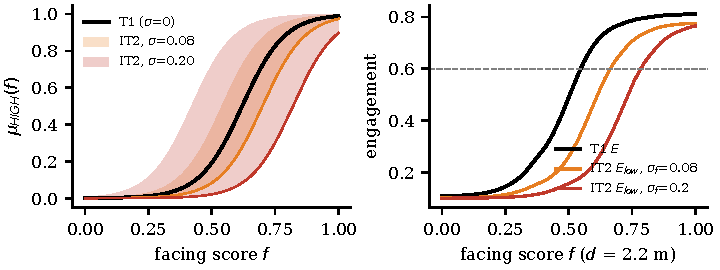
\includegraphics[width=\linewidth]{figures/fou}
\caption{Left: the facing-HIGH set for three uncertainty levels. Right:
engagement versus facing score for a person at 2.2\,m. As uncertainty grows,
the IT2 lower bound needs a clearer view before it crosses the acceptance
threshold (dashed).}
\label{fig:fou}
\end{figure}

\subsection{Layer 2: decision and arbitration}
A gesture with label $\ell$ and confidence $c$ from person $p$ is accepted if
\begin{equation}
\Elow(p,t)\ge\theta_E(\ell)\quad\wedge\quad c\ge\theta_c,
\label{eq:decision}
\end{equation}
with $\theta_E=0.60$ for motion commands, a lower $\theta_E=0.45$ for STOP
(a safety bias), and $\theta_c=0.45$. The Type-1 policy uses its crisp $E$.
A decision must persist for three frames. If several people are accepted at
once, STOP wins; otherwise the most engaged person wins. Commands are sent as
velocity set-points at 10\,Hz with a 0.3\,m/s cap, and the robot stops 0.5\,s
after the last accepted gesture. All thresholds were set on a development
recording and frozen before the test sessions.

\section{Experimental Setup}
\label{sec:experiments}

\paragraph{Platform.} \TODO{Unitree Go2 model, camera resolution and frame
rate, laptop CPU, achieved fps.}

\paragraph{Participants and scenarios.} \TODO{P participants (roles rotated),
two locations, consent.} Six stationary scenarios: single commander (S1);
bystanders gesturing to each other beside the commander (S2); commander and
bystander gesturing simultaneously (S3); commander turning to gesture to a
friend and back (S4); two people commanding at once (S5); bystanders walking
past (S6). Three walking scenarios, with the robot driven by the IT2 policy:
commander drives the robot among bystanders (W1), a bystander gestures nearby
while it walks (W2), and people cross between robot and commander (W3).
\TODO{number of takes, total minutes.}

\paragraph{Policies.} All policies run on the same per-person features in the
same frame (one drives the robot; all are logged): \emph{gesture-only} (any
confident command gesture), \emph{nearest person}, \emph{gaze-only} (gesture
from anyone whose gaze/facing exceeds a threshold), a \emph{learned} baseline
(logistic regression on the same features, trained on the development split),
\emph{Type-1} and \emph{IT2} engagement gates.

\paragraph{Labels and metrics.} A gesture episode is one tracked person
holding one command gesture for at least three frames. Two annotators
independently labelled every episode as addressed to the robot or not
(Cohen's $\kappa=$\RES{}~\cite{cohen1960kappa}); disagreements were resolved
by a third. The \emph{bystander false-trigger rate} is the fraction of
not-addressed episodes a policy would execute; \emph{commander recall} is the
fraction of addressed episodes it executes. We report 95\% Wilson
intervals~\cite{wilson1927probable}, compare IT2 and Type-1 on paired
episodes with McNemar's test~\cite{mcnemar1947note}, and sweep $\theta_E$ to
obtain false-trigger versus recall curves.

\paragraph{Distance sources.} \TODO{Ablation: the IT2 gate with $\sigma_d$
from a monocular estimate, from RGB-D depth, and (if available) from LiDAR--camera
fusion; depth/LiDAR agreement on calibration takes.}

\section{Results}
\label{sec:results}

\begin{table}[t]
\centering
\caption{Bystander false-trigger rate (FT, lower is better) and commander
recall (higher is better) with 95\% Wilson intervals.
\RES{numbers from results/table}}
\label{tab:main}
\setlength{\tabcolsep}{4pt}
\begin{tabular}{lcccc}
\toprule
& \multicolumn{2}{c}{Stationary} & \multicolumn{2}{c}{Walking}\\
\cmidrule(lr){2-3}\cmidrule(lr){4-5}
Policy & FT $\downarrow$ & Recall $\uparrow$ & FT $\downarrow$ & Recall $\uparrow$\\
\midrule
Gesture only      & \RES{} & \RES{} & \RES{} & \RES{}\\
Nearest person    & \RES{} & \RES{} & \RES{} & \RES{}\\
Gaze only         & \RES{} & \RES{} & \RES{} & \RES{}\\
Learned (LR)      & \RES{} & \RES{} & \RES{} & \RES{}\\
Type-1 engagement & \RES{} & \RES{} & \RES{} & \RES{}\\
\textbf{IT2 engagement (ours)} & \RES{} & \RES{} & \RES{} & \RES{}\\
\bottomrule
\end{tabular}
\end{table}

\TODO{Main result paragraph (Table~\ref{tab:main}).}

\TODO{Operating curves: FT vs.\ recall when sweeping $\theta_E$; FT at 90\%
recall.}

\TODO{Where IT2 helps: results split by measured uncertainty (low/high
$\sigma$), distance and occlusion; McNemar $p$.}

\TODO{Ablations: without gaze, facing only, distance only, without approach
speed; FOU scale $k$; noise injection.}

\TODO{Closed loop: unintended robot motions per minute in walking takes;
runtime.}

\section{Discussion and Limitations}
\label{sec:discussion}

\TODO{What the results mean: which cue carried most of the information; why
nearest-person fails when a bystander is closer; where IT2 helps and what it
costs in recall.}

\paragraph{Limitations.} Distance comes from a single RGB-D camera; the
robot's built-in LiDAR is \TODO{not fused at run time / fused offline only}. Gaze is only informative
at short range. The study uses a small number of participants in
\RES{two} indoor locations, with labels from two annotators, so the results are
indicative rather than definitive. Rule parameters were designed by hand and
tuned on a single development recording.

\paragraph{Future work.} LiDAR--camera fusion for distance, learning the rule
parameters and the FOU scale from data, extending the gate to voice and
pointing, and a user study of perceived safety and trust.

\section{Conclusion}
\label{sec:conclusion}

Asking \emph{whose} gesture it is, and whether that person is addressing the
robot, is a small change to a gesture interface that matters in crowds. We
presented a per-person fuzzy engagement gate for a quadruped robot in which
an Interval Type-2 footprint of uncertainty follows measured perception
uncertainty, so the robot obeys its commander while asking for more evidence
from people it cannot see clearly. \RES{One sentence on the main result.}


% Acknowledgements are removed for double-blind review.
% \begin{credits}
% \subsubsection{\ackname} This work was supported by WSO2 ...
% \end{credits}

\bibliographystyle{splncs04}
\bibliography{references}

\end{document}
